
\section{Introduction}

	\defn{Web Application}{is a distributed information management system. In
essence it is an application , usually spread around several machines, which allows
users to query and manipulate data, and which is then displayed via the browser}

	\rem{The distinction between a website and a web app is less clear nowadays,
but the main feature of a web app seems to be its interactive nature, as opposed
to the more expository nature of simple websites}

	\defn{Distributed Information Management System (DIM)}{a
group of machines working together but appearing to the user as a single entity.
These systems have major advantages, such as concurrent and independent
operation. One machine can fail or be upgraded without the system failing}

\subsubsection{Architecture}

	\par{A common system architecture for a DIM is represented in the diagram
below. Web development has a wide range of tools and new frameworks and
languages come into being every other week. In this class, we'll focus on the
tools listed below but in general each tool group performs certain tasks which
are essential to each bit of the system}

	\rem{Most web apps follow a 3-tier architecture : Presentation, Application,
			Data. The rango app will also include an external service , the Bing
	search API}

	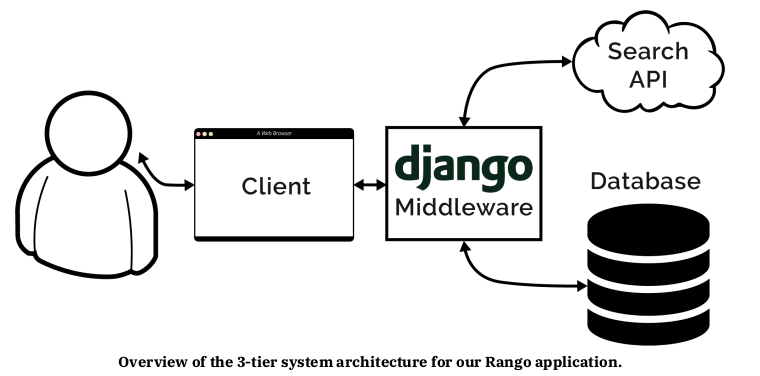
\includegraphics[width=\textwidth]{3arch}
	\defn{User}{machine or person which initiates contact with the client}

	\defn{Client}{program sitting on the user device which sends/accepts
requests/responses and acts on the messages by communicating to them the user
and/or by altering state in some way}

	\rem{A request is usually done via \texttt{HTTP} where the data to be sent is
	embedded, and responses are also sent via \texttt{HTTP} with content usually
	delivered in a markup language like \texttt{XHTML} or \texttt{JSON}}

	\defn{Middleware}{Responsible for accepting and sending responses on server
side and for coordinating messages}

	\rem{In this course we'll be using Django}

	\rem{The database is usually kept in a separate node}


\subsubsection{Tools Covered}

		\mymarginpar{Proficiency expected}
		\begin{multicols}{2}
				\begin{enumerate}
					\item Python
					\item Django
					\item HTML/CSS
					\item HTTP GET/POST
					\item XML/XHTML/JSON
					\item JS
					\item JQuery
					\item AJAX
					\item Github
					\item Pip
					\item PythonAywhere
					\item IDLE
					\item Venv
					\item Draw.io
				\end{enumerate}
		\end{multicols}

	\section{Development Environment}

	\key{Git}{package management}{pip}{IDE}{Django}{SE best
	practices}{repository}{pip}{virtual environment}{version control}

	\par{Over the years web applications' development adopted many practices
			from software engineering, in order to maximize productivity. It is
			essential to setup your development environment appropriately.Below
			we explore common tools and practices widely used in industry}

	\subsection{Version Control Systems}

	\defn{VCS}{software which makes tracking and managing changes to documents
	easy}

	\defn{Repository}{where copies of a project/file being tracked are stored}

	\defn{Snapshot}{the state of the file at a point in time}

	\par{VC is widely used not only in industry but in personal and open-source
			projects. It's main advantages being the fact that it makes
			collaboration easy since everyone in a team can read from and write
			to the same repository ; the fact that it allows for several
			working versions of a project to be stored separately without having
			to save a copy of every single file (instead pointers for existing
			files are simply stored with every new commit); and also the fact
			that it prevents against loss of code, specially when stored in a
	remote repository}

	\subsection{Git}

	\par{The most widely used VCS is Git , invented by Linus Torvalds in 2005.
		Before, the most widely used software was SVN. They differ mainly in how
		changes are distributed to the shared version. SVN uses a single central
		repository, which means that your data is stored in a single place in a
		server. Git, on the other hand, allows developers to keep a local copy
		of the shared repository, and allows for greater granularity when
		deciding which changes to apply and when, by offering a staging area.
		When ready to share the changes, developers \ita{push} their local repo
to the \ita{remote}/shared one}

	\subsubsection{Git Workflow}

	\par{Git uses 3 local spaces:}

	\begin{itemize}
			\setlength\itemsep{0.5em}
			\item[]\textbf{Workspace} is your working directory, where \texttt{.git} is
			created when initializing the repository, along with some other
			needed files for version control

			\item[]\textbf{Index} is the staging area, where files being tracked are
			added prior to commiting. It consists of a binary file with a list
			of all the files in the workspace

			\item[]\textbf{Local Repository} is where the actual copies of the files
			for all branches (both local and remote) exist
	\end{itemize}

	\begin{figure}[H]
			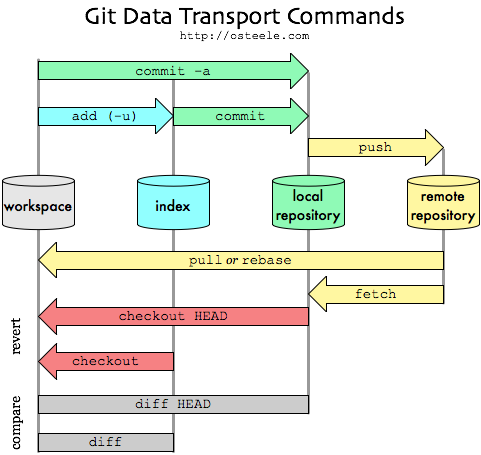
\includegraphics[height=0.35\textheight , width=\textwidth]{git.png}
	\end{figure}

	\rem{Git mantra : \ita{"commit early, commit often"}}

	\rem{See \cite{knowBase} for further details}


\subsection{Package Management}

	\defn{Package Manager}{software tool that automates the process of
	installing, upgrading and configuring software libraries}

	\par{Prior to the existence of package managers, running other
			developers' apps could be incredibly difficult ; not because there
			was something inherently wrong in its code base, but because as apps
			became more complex, they relied on public libraries, each with
			their own specific version, and keeping track of it all and setting
			them up individually was not the easiest of tasks
			\cite{ovens} . PMs help overcome this difficulties by partially
	recreating the creator's environment. Hence, the process becomes
	\ita{defined} , since a list of the required packages is distributed along
	with the rest of the software ; \ita{repeatable} and \ita{exportable} since
	the list of the required packages and their versions is passed onto the
	package manager and can be easily exported}

	\rem{In this course we'll be using
			\href{https://pypi.org/project/pip/}{pip} the \ita{de facto}
	PM for python-based apps}

\subsection{Virtual Environments}

	\defn{Virtual Environment}{a local
environment that is configured to provide access
to libraries, settings, hardware}

	\par{Installing software system-wide is not considered a best-practice.
			Often, environments will clash, given that, as discussed above,
			different apps might require different versions of the same
			software. In order to avoid this, it is best to setup a virtual
			environment for your project. This way we satisfy each project
	dependencies, while avoiding system-wide conflicts}

	\rem{Anaconda will be used in the lab machines. Use VirtualEnv with
	VirtualEnvWrapper in yours}
